%%%%%%%%%%%%%%%%%%%%%%%%%%%%%%%%%%%%%%%%%%%%%%%%%%%%%%%%%%%%%%%%%%%%%%%%%%%

\documentclass[a4paper,oneside,12pt]{article}
\usepackage{mystyle}

\begin{document}

\title{\Large\bf Quadratic functions}
\author{%%
  Minh Van Nguyen \\
  \url{mvngu@gmx.com}
}
\date{\today}
\maketitle

\begin{packeditem}
\item Factoring quadratic function.

\item Completing the square.

\item Application: gravity and displacement of projectile.

\item Area under a quadratic function.
\end{packeditem}


%%%%%%%%%%%%%%%%%%%%%%%%%%%%%%%%%%%%%%%%%%%%%%%%%%%%%%%%%%%%%%%%%%%%%%%%%%%

\section{General form}
\label{sec:general_form}

A \emph{quadratic function} is an equation of the form
%%
\begin{equation}
\label{eqn:general_quadratic_function}
f(x)
=
ax^2 + bx + c
\end{equation}
%%
where $\triple{a}{b}{c} \in \RR$ are known constants such that
$a \neq 0$ and $x$ is a variable that can be any real number.  What
does the function $f(x)$ look like?

As an example, set $a = 1$ and $b = c = 0$ in
\Equation{eqn:general_quadratic_function} so that you have
$f(x) = x^2$.  Let's calculate the function value for
$x = \sextuple{-4}{-3}{-2}{2}{3}{4}$.  Note that you have
\[
f(2) = f(-2) = 4,
%%
\quad
%%
f(3) = f(-3) = 9,
%%
\quad
%%
f(4) = f(-4) = 16.
\]
Plot these points on one set of coordinate axes and draw a line
through the points to get the graph in \Figure{fig:quadratic_a_1}.
Note that $f(0) = 0$ so the graph of $f(x) = x^2$ touches the origin.
The general shape of the graph of
\Equation{eqn:general_quadratic_function} looks like the beak of a
duck~(or a nose) and the usual name for this is a \emph{parabola}.

\begin{figure}[!htbp]
\centering
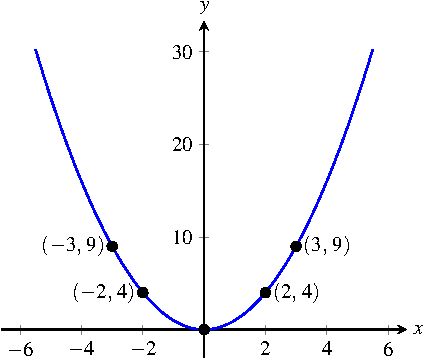
\includegraphics[scale=1.2]{image/07/a-1.pdf}
\caption{%%
  A graph of the function $f(x) = x^2$.  The general shape of the
  graph is called a \emph{parabola}.
}
\label{fig:quadratic_a_1}
\end{figure}

Generally speaking, how would you draw the graph of
\Equation{eqn:general_quadratic_function}?  One way is to start at the
tip of the parabola and choose a few values of $x$ that are equally
spaced.  If the tip of the parabola is $\tuple{a}{b}$, the following
values of $x$
\[
\septuple{a-3}{a-2}{a-1}{a}{a+1}{a+2}{a+3}
\]
should usually be good enough for a rough sketch of the graph of
\Equation{eqn:general_quadratic_function}.  Of course, you still need
to calculate the function values $f(a-3)$, $f(a-2)$, $f(a-1)$,
$f(a+1)$, $f(a+2)$, and $f(a+3)$.  Note that the graph of the
quadratic function $f(x)$ is symmetric about the tip point
$\tuple{a}{b}$.  This means that
\[
f(a+1) = f(a-1),
%%
\quad
%%
f(a+2) = f(a-2),
%%
\quad
%%
f(a+3) = f(a-3)
\]
and so you only need to calculate three function values, not six.
The above strategy is illustrated
in \Figure{fig:sketch_parabola}.

\begin{figure}[!htbp]
\centering
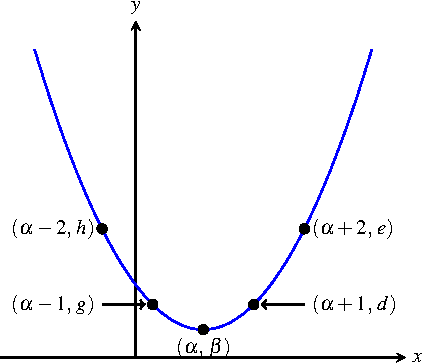
\includegraphics[scale=1.2]{image/07/a1-bminus4-c10.pdf}
\caption{%%
  Sketching the graph of a quadratic function.  First, locate the tip
  $\tuple{a}{b}$ of the function.  From there, spread outward with a
  few points.  Finally, you connect the dots.
}
\label{fig:sketch_parabola}
\end{figure}

The problem now is: How do you calculate the tip of the parabola?  If
you have a quadratic function of the form $f(x) = ax^2 + bx + c$, the
tip of the function is located at the $x$-coordinate
%%
\begin{equation}
\label{eqn:parabola_tip_x_coordinate}
x
=
-\frac{b}{2a}.
\end{equation}
%%
Substitute \Expression{eqn:parabola_tip_x_coordinate} into the
function $f(x)$ to obtain the corresponding $y$-coordinate.  For now,
do not worry about how \Expression{eqn:parabola_tip_x_coordinate} was
derived.  This will be shown later on.

\begin{example}
\label{ex:quadratic_graph_a1_b1_c1}
Sketch the graph of the quadratic function $f(x) = x^2 + x + 1$.
\end{example}

\begin{solution}
The first thing you should do is determine the tip point.  You have
the values $a = 1$ and $b = 1$.  Use
\Expression{eqn:parabola_tip_x_coordinate} to see that the
$x$-coordinate of the tip point is
%%
\begin{align*}
x
&=
-\frac{1}{2 \times 1} \\[4pt]
&=
-\frac{1}{2}
\end{align*}
%%
and the $y$-coordinate of the tip point is
%%
\begin{align*}
y
&=
f(-1/2) \\[4pt]
&=
\parenthesis*{-\frac{1}{2}}^2 + \parenthesis*{-\frac{1}{2}} + 1 \\[4pt]
&=
\frac{1}{4} - \frac{1}{2} + 1 \\[4pt]
&=
\frac{1}{4} - \frac{2}{4} + \frac{4}{4} \\[4pt]
&=
\frac{1 - 2 + 4}{4} \\[4pt]
&=
\frac{3}{4}.
\end{align*}
%%
Thus the tip of the parabola is the point
$\tuple{-\frac{1}{2}}{\frac{3}{4}}$.  Next, choose the $x$-coordinates
%%
\begin{equation}
\label{eqn:a1_b1_c1_x_coordinates}
\frac{1}{2} = -\frac{1}{2} + 1,
%%
\qquad
%%
\frac{3}{2} = -\frac{1}{2} + 2,
%%
\qquad
%%
\frac{5}{2} = -\frac{1}{2} + 3
\end{equation}
%%
whose corresponding $y$-coordinates are
$\triple{\frac{7}{4}}{\frac{19}{4}}{\frac{39}{4}}$.  These three
$y$-coordinates also correspond to the $x$-coordinates
$\triple{-\frac{3}{2}}{-\frac{5}{2}}{-\frac{7}{2}}$ and so you have
\[
f(1/2) = f(-3/2),
%%
\quad
%%
f(3/2) = f(-5/2),
%%
\quad
%%
f(5/2) = f(-7/2).
\]
Plot the above seven points, connect the dots, and you get the graph
shown in \Figure{fig:quadratic_graph_a1_b1_c1}.
\end{solution}

\begin{figure}[!htbp]
\centering
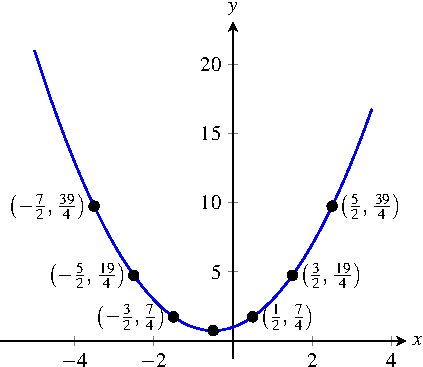
\includegraphics[scale=1.2]{image/07/a1-b1-c1.pdf}
\caption{%%
  A graph of the quadratic function $f(x) = x^2 + x + 1$.  The tip of
  the function is at the point $\tuple{-\frac{1}{2}}{\frac{3}{4}}$.
}
\label{fig:quadratic_graph_a1_b1_c1}
\end{figure}

\begin{exercise}
For the $x$-coordinates~\eqref{eqn:a1_b1_c1_x_coordinates} in
\Example{ex:quadratic_graph_a1_b1_c1}, verify that the corresponding
$y$-coordinates are
$\triple{\frac{7}{4}}{\frac{19}{4}}{\frac{39}{4}}$.
\end{exercise}
%%
\ifbool{showSolution}{
\begin{solution}
The quadratic function is $f(x) = x^2 + x + 1$.  For $x = 1/2$ you have
%%
\begin{align*}
f(1/2)
&=
\parenthesis*{\frac{1}{2}}^2 + \frac{1}{2} + 1 \\[4pt]
&=
\frac{1}{4} + \frac{1}{2} + 1 \\[4pt]
&=
\frac{1}{4} + \frac{2}{4} + \frac{4}{4} \\[4pt]
&=
\frac{7}{4}.
\end{align*}
%%
For $x = 3/2$ you have
%%
\begin{align*}
f(3/2)
&=
\parenthesis*{\frac{3}{2}}^2 + \frac{3}{2} + 1 \\[4pt]
&=
\frac{9}{4} + \frac{3}{2} + 1 \\[4pt]
&=
\frac{9}{4} + \frac{6}{4} + \frac{4}{4} \\[4pt]
&=
\frac{19}{4}.
\end{align*}
%%
For $x = 5/2$ you have
%%
\begin{align*}
f(5/2)
&=
\parenthesis*{\frac{5}{2}}^2 + \frac{5}{2} + 1 \\[4pt]
&=
\frac{25}{4} + \frac{5}{2} + 1 \\[4pt]
&=
\frac{25}{4} + \frac{10}{4} + \frac{4}{4} \\[4pt]
&=
\frac{39}{4}.
\end{align*}
\end{solution}
}{}

\begin{exercise}
Sketch the graph of the function $f(x) = x^2 - 2x + 2$.
\end{exercise}
%%
\ifbool{showSolution}{
\begin{solution}
First, you determine the tip point.  You have $a = 1$ and $b = -2$.
Use \Expression{eqn:parabola_tip_x_coordinate} to see that the
$x$-coordinate of the tip point is
%%
\begin{align*}
x
&=
-\frac{-2}{2 \times 1} \\[4pt]
&=
\frac{2}{2} \\[4pt]
&=
1.
\end{align*}
%%
The $y$-coordinate of the tip point is
%%
\begin{align*}
f(1)
&=
1^2 - 2(1) + 2 \\[4pt]
&=
1 - 2 + 2 \\[4pt]
&=
1.
\end{align*}
%%
Then the tip of the parabola is the point $\tuple{1}{1}$.  Next,
choose the following values for $x$:
\[
2 = 1 + 1,
%%
\qquad
%%
3 = 1 + 2,
%%
\qquad
%%
4 = 1 + 3.
\]
The corresponding $y$ values are
\[
f(2) = f(0) = 2,
%%
\qquad
%%
f(3) = f(-1) = 5,
%%
\qquad
%%
f(4) = f(-2) = 10.
\]
Plot the above seven points to obtain the graph shown in
\Figure{fig:graph_a1_bminus2_c2}.

\begin{figure}[!htbp]
\centering
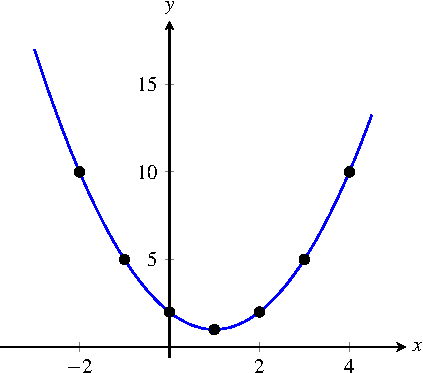
\includegraphics[scale=1.2]{image/07/a1-bminus2-c2.pdf}
\caption{%%
  A graph of the function $f(x) = x^2 - 2x + 2$.  The tip of the
  parabola is the point $\tuple{1}{1}$.
}
\label{fig:graph_a1_bminus2_c2}
\end{figure}
\end{solution}
}{}


%%%%%%%%%%%%%%%%%%%%%%%%%%%%%%%%%%%%%%%%%%%%%%%%%%%%%%%%%%%%%%%%%%%%%%%%%%%

\section{Quadratic formula}
\label{sec:quadratic_formula}

Given a quadratic function $f(x) = ax^2 + bx + c$, sometimes a problem
requires you to determine the values of $x$ such that $f(x) = 0$.
Those values of $x$ for which the equation $f(x) = 0$ is true are
called the \emph{roots} of $f(x)$.  When you need to find the roots of
$f(x)$, the \emph{quadratic formula} is guaranteed to provide you with
at least one root.  But what is the quadratic formula and how is it
derived?

\begin{exercise}
\label{ex:completing_the_square}
Let $\pair{a}{b} \in \RR$ be constants such that $a \neq 0$ and let
$x$ be a real variable.  Show that
\[
\parenthesis*{x + \frac{b}{2a}}^2
=
x^2 + \frac{b}{a} x + \parenthesis*{\frac{b}{2a}}^2.
\]
\end{exercise}
%%
\ifbool{showSolution}{
\begin{solution}
Use the distributive laws to expand
$\parenthesis*{x + \frac{b}{2a}}^2$ and you get
%%
\begin{align*}
\parenthesis*{x + \frac{b}{2a}}^2
&=
\parenthesis*{x + \frac{b}{2a}} \parenthesis*{x + \frac{b}{2a}} \\[4pt]
&=
x \parenthesis*{x + \frac{b}{2a}}
+
\frac{b}{2a} \parenthesis*{x + \frac{b}{2a}} \\[4pt]
&=
x^2 + \frac{b}{2a} x + \frac{b}{2a} x + \parenthesis*{\frac{b}{2a}}^2 \\[4pt]
&=
x^2 + 2 \times \frac{b}{2a} x + \parenthesis*{\frac{b}{2a}}^2 \\[4pt]
&=
x^2 + \frac{b}{a} x + \parenthesis*{\frac{b}{2a}}^2
\end{align*}
%%
as required.
\end{solution}
}{}

\begin{exercise}
\label{ex:completing_the_square_redux}
Let $x$ be a real variable and suppose $\triple{a}{b}{c} \in \RR$ are
constants such that $a \neq 0$.  Show that the expression
\[
\parenthesis*{
  x + \frac{b}{2a}
}^2
=
\frac{
  b^2 - 4ac
}{
  4a^2
}
\]
can also be written as $(2ax + b)^2 = b^2 - 4ac$.
\end{exercise}
%%
\ifbool{showSolution}{
\begin{solution}
The statement of the problem assumes that the expression
\[
\parenthesis*{
  x + \frac{b}{2a}
}^2
=
\frac{
  b^2 - 4ac
}{
  4a^2
}
\]
is true.  For the sake of argument, you can assume that the expression
is true.  Multiplying both sides by $4a^2$ produces the expression
%%
\begin{equation}
\label{eqn:complete_the_square_no_denominator}
4a^2 \parenthesis*{x + \frac{b}{2a}}^2
=
b^2 - 4ac
\end{equation}
%%
where the left-hand side can be factored as
%%
\begin{equation}
\label{eqn:complete_the_square_factored}
\begin{aligned}
4a^2 \parenthesis*{x + \frac{b}{2a}}^2
&=
(2a)^2 \parenthesis*{x + \frac{b}{2a}}^2 \\[4pt]
&=
\squarebracket*{2a \parenthesis*{x + \frac{b}{2a}}}^2 \\[4pt]
&=
\parenthesis*{2ax + 2a \times \frac{b}{2a}}^2 \\[4pt]
&=
\parenthesis*{2ax + b}^2.
\end{aligned}
\end{equation}
%%
Conclude from
\Expressions{eqn:complete_the_square_no_denominator}{eqn:complete_the_square_factored}
that $(2ax + b)^2 = b^2 - 4ac$.
\end{solution}
}{}

\begin{exercise}
Let $a \in \RR$ and consider the numbers $\pm\sqrt{a}$.  Here the
symbol ``$\pm$'' means that you have both of $\sqrt{a}$ and
$-\sqrt{a}$.  If $x = \pm\sqrt{a}$, prove that $x^2 = a$.
\end{exercise}
%%
\ifbool{showSolution}{
\begin{solution}
You must prove two statements:
%%
\begin{packedenumeral}
\item\label{case:x_sqrt_a_implies_x_squared_a}
  If $x = \sqrt{a}$ then $x^2 = a$.

\item\label{case:x_minus_sqrt_a_implies_x_squared_a}
  If $x = -\sqrt{a}$ then $x^2 = a$.
\end{packedenumeral}
%%
First, let's prove \Statement{case:x_sqrt_a_implies_x_squared_a}.  If
$x = \sqrt{a}$, then you can square both sides of the equation to get
$x^2 = (\sqrt{a})^2$.  Since $\sqrt{a} = a^{1/2}$, then you can write
the expression $x^2 = (\sqrt{a})^2$ as
%%
\begin{equation}
\label{eqn:x_sqrt_a_implies_x_squared_a}
\begin{aligned}
x^2
&=
(\sqrt{a})^2 \\[4pt]
&=
(a^{1/2})^2 \\[4pt]
&=
a^{2/2} \\[4pt]
&=
a.
\end{aligned}
\end{equation}
%%
Finally, let's prove
\Statement{case:x_minus_sqrt_a_implies_x_squared_a}.  If
$x = -\sqrt{a}$, then squaring both sides of the equation results in
%%
\begin{align*}
x^2
&=
\bigparen{(-1)\sqrt{a}}^2 \\[4pt]
&=
(-1)^2 (\sqrt{a})^2 \\[4pt]
&=
(\sqrt{a})^2.
\end{align*}
%%
The latter equation can be simplied to $x^2 = a$ by using
\Expression{eqn:x_sqrt_a_implies_x_squared_a}.  Therefore if
$x = \pm\sqrt{a}$ then you have $x^2 = a$.
\end{solution}
}{}

\begin{exercise}
\label{ex:x_squared_a_implies_plus_minus_sqrt_a}
If $a$ is a real number such that $x^2 = a$, prove that
$x = \pm\sqrt{a}$.
\end{exercise}
%%
\ifbool{showSolution}{
\begin{solution}
You have two statements to prove:
%%
\begin{packedenumeral}
\item\label{case:x_squared_a_sqrt_a}
  If $a \in \RR$ such that $x^2 = a$, then $x = \sqrt{a}$.

\item\label{case:x_squared_a_minus_sqrt_a}
  If $a \in \RR$ such that $x^2 = a$, then $x = -\sqrt{a}$.
\end{packedenumeral}
%%
First, let's prove \Statement{case:x_squared_a_sqrt_a}.  You know that
$x^2 = a$ and the square root of any number $c \in \RR$ can be written
as $\sqrt{c} = c^{1/2}$.  Taking the square root of both sides of the
equation $x^2 = a$ and you get $(x^2)^{1/2} = a^{1/2}$, which can also
be written as $x^{2/2} = a^{1/2}$.  The latter equation simplifies to
$x = \sqrt{a}$ because $x^{2/2} = x^1 = x$.

Finally, let's prove \Statement{case:x_squared_a_minus_sqrt_a}.  You
know that $x^2 = a$ and since $a = (-1)^2 a$, you can also write
$x^2 = (-1)^2 a$.  Take the square root of both sides of the last
equation to get $(x^2)^{1/2} = \bigparen{(-1)^2 a}^{1/2}$, which can
be written as $x^{2/2} = (-1)^{2/2} a^{1/2}$.  Use the fact that
$(-1)^{2/2} = (-1)^1 = -1$ to write $x = -\sqrt{a}$.
\end{solution}
}{}

First, let's derive the quadratic formula.  When you write $f(x) = 0$,
it is the same as writing $ax^2 + bx + c = 0$.  When you require a
value of $x$ such that $f(x) = 0$, i.e.~a root of $f(x)$, what you
really want is to solve the equation $ax^2 + bx + c = 0$ for $x$.  In
the last equation, dividing each term by $a$ results in the equivalent
expression
\[
x^2 + \frac{b}{a} x + \frac{c}{a}
=
0.
\]
Now move the term $c/a$ to the right-hand side to obtain
%%
\begin{equation}
\label{eqn:quadratic_formula_factor_LHS}
x^2 + \frac{b}{a} x
=
-\frac{c}{a}.
\end{equation}
%%
The problem now is to factor the left-hand side of
\Equation{eqn:quadratic_formula_factor_LHS}.  From
\Exercise{ex:completing_the_square} you know that the square
$\parenthesis*{x + \frac{b}{2a}}^2$ can be expanded to become
\[
\parenthesis*{x + \frac{b}{2a}}^2
=
x^2 + \frac{b}{a} x + \parenthesis*{\frac{b}{2a}}^2
\]
where the expression $x^2 + \frac{b}{a} x$ is the same as the
left-hand side of \Equation{eqn:quadratic_formula_factor_LHS}.  Adding
$\parenthesis*{\frac{b}{2a}}^2$ to both sides of
\Equation{eqn:quadratic_formula_factor_LHS} results in
%%
\begin{align*}
x^2 + \frac{b}{a} x + \parenthesis*{\frac{b}{2a}}^2
&=
-\frac{c}{a} + \parenthesis*{\frac{b}{2a}}^2 \\[4pt]
&=
-\frac{c}{a} + \frac{b^2}{4a^2} \\[4pt]
&=
-\frac{c}{a} \times \frac{4a}{4a} + \frac{b^2}{4a^2} \\[4pt]
&=
-\frac{4ac}{4a^2} + \frac{b^2}{4a^2} \\[4pt]
&=
\frac{
  b^2 - 4ac
}{
  4a^2
}.
\end{align*}
%%
Now use \Exercise{ex:completing_the_square} to factor the left-hand
side of the latter expression and you can write
\Equation{eqn:quadratic_formula_factor_LHS} as
\[
\parenthesis*{x + \frac{b}{2a}}^2
=
\frac{
  b^2 - 4ac
}{
  4a^2
}.
\]
By \Exercise{ex:completing_the_square_redux} this expression is the
same as the equation $(2ax + b)^2 = b^2 - 4ac$.  Use
\Exercise{ex:x_squared_a_implies_plus_minus_sqrt_a} to write the last
equation as $2ax + b = \pm\sqrt{b^2 - 4ac}$.  Solve for $x$ and you
obtain
%%
\begin{align*}
x
&=
\frac{
  -b \pm \sqrt{b^2 - 4ac}
}{
  2a
}
\end{align*}
%%
which is called the \emph{quadratic formula}.  The above can be
summarised as follows.

\begin{theorem}
\label{thm:quadratic_formula}
\textbf{Quadratic formula.}
Let $\triple{a}{b}{c} \in \RR$ such that $a \neq 0$ and consider the
quadratic function $f(x) = ax^2 + bx + c$.  The roots of $f(x)$ can be
written as
%%
\begin{equation}
\label{eqn:quadratic_formula}
x
=
\frac{
  -b \pm \sqrt{b^2 - 4ac}
}{
  2a
}.
\end{equation}
\end{theorem}

What does the quadratic \Formula{eqn:quadratic_formula} mean?  How do
you make sense of the equation?  Let's assume you have a quadratic
function $f(x) = ax^2 + bx + c$ with $\triple{a}{b}{c}$ being real
numbers such that $a \neq 0$.
Expression~\eqref{eqn:quadratic_formula} states that there are values
of $x$ such that $f(x) = 0$ and those values of $x$ can be written as
\[
x
=
\frac{
  -b + \sqrt{b^2 - 4ac}
}{
  2a
}
%%
\qquad
\text{and}
\qquad
%%
x
=
\frac{
  -b - \sqrt{b^2 - 4ac}
}{
  2a
}.
\]
How can you use the quadratic formula to help you sketch the graph of
a quadratic function? In the graph of $f(x)$, the $x$-intercept is
obtained by setting $f(x) = 0$ and solving the last equation for $x$.
The whole point of \Theorem{thm:quadratic_formula} is to help you
calculate the $x$-intercepts of a quadratic function.
\Theorem{thm:quadratic_formula} also says that a quadratic function
has at most two $x$-intercepts.  The next example should help to
clarify the theory.

\begin{example}
Sketch the graph of the function $f(x) = x^2 - x - 2$.
\end{example}

\begin{solution}
You have the values $a = 1$, $b = -1$, and $c = -2$.  You can use
three points to draw the graph of $f(x)$.  The first point is the tip
of the parabola.  The other two points are the $x$-intercepts of
$f(x)$.

First, let's determine the tip point.  From
\Equation{eqn:parabola_tip_x_coordinate} you know that the tip of the
parabola occurs at the $x$-coordinate
%%
\begin{align*}
x
&=
-\frac{-1}{2 \times 1} \\[4pt]
&=
\frac{1}{2}.
\end{align*}
%%
Then the $y$-coordinate of the tip point is
%%
\begin{align*}
y
&=
f(1/2) \\[4pt]
&=
\parenthesis*{\frac{1}{2}}^2 - \frac{1}{2} - 2 \\[4pt]
&=
\frac{1}{4} - \frac{2}{4} - \frac{8}{4} \\[4pt]
&=
\frac{1 - 2 - 8}{4} \\[4pt]
&=
-\frac{9}{4}.
\end{align*}
%%
Thus the tip of the parabola occurs at the point
$\tuple{\frac{1}{2}}{-\frac{9}{4}}$.

Next, let's calculate the $x$-intercepts of $f(x)$.  From
\Equation{eqn:quadratic_formula} you know that one of the
$x$-intercepts occurs at
%%
\begin{align*}
x
&=
\frac{
  -(-1) + \sqrt{(-1)^2 - 4(1)(-2)}
}{
  2(1)
} \\[4pt]
&=
\frac{
  1 + \sqrt{1 + 8}
}{
  2
} \\[4pt]
&=
\frac{
  1 + \sqrt{9}
}{
  2
} \\[4pt]
&=
\frac{
  1 + 3
}{
  2
} \\[4pt]
&=
2.
\end{align*}
%%
The other $x$-intercept occurs at
%%
\begin{align*}
x
&=
\frac{
  -(-1) - \sqrt{(-1)^2 - 4(1)(-2)}
}{
  2(1)
} \\[4pt]
&=
\frac{
  1 - \sqrt{9}
}{
  2
} \\[4pt]
&=
\frac{
  1 - 3
}{
  2
} \\[4pt]
&=
-1.
\end{align*}
%%
In other words, you have two different $x$-intercepts that occur at
the points $\tuple{2}{0}$ and $\tuple{-1}{0}$.  Plot the tip point and
the two $x$-intercepts on one set of coordinate axes, draw a line
through the points, and you obtain the graph in
\Figure{fig:a1_bminus1_cminus2}.
\end{solution}

\begin{figure}[!htbp]
\centering
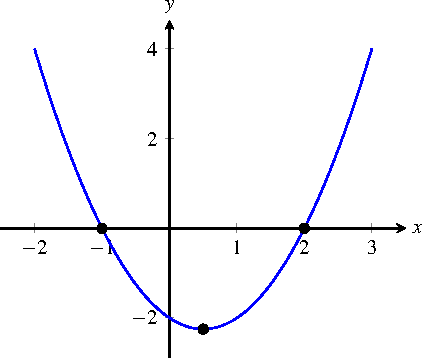
\includegraphics[scale=1]{image/07/a1-bminus1-cminus2.pdf}
\caption{%%
  Graph of the function $f(x) = x^2 - x - 2$ through three points.
}
\label{fig:a1_bminus1_cminus2}
\end{figure}

\begin{exercise}
Sketch the graph of $f(x) = -2x^2 + x + 3$.
\end{exercise}
%%
\ifbool{showSolution}{
\begin{solution}
You have the values $a = -2$, $b = 1$, and $c = 3$.  You can draw the
graph of $f(x) = -2x^2 + x + 3$ by using three points: the tip of the
parabola and the two $x$-intercepts.

First, let's calculate the tip point of the parabola.  Use
\Equation{eqn:parabola_tip_x_coordinate} to see that the tip point
occurs at the $x$-coordinate
%%
\begin{align*}
x
&=
-\frac{1}{2(-2)} \\[4pt]
&=
\frac{1}{4}.
\end{align*}
%%
The $y$-coordinate of the tip point is
%%
\begin{align*}
y
&=
f(1/4) \\[4pt]
&=
-2\parenthesis*{\frac{1}{4}}^2 + \frac{1}{4} + 3 \\[4pt]
&=
-2 \times \frac{1}{16} + \frac{4}{16} + 3 \\[4pt]
&=
\frac{4 - 2}{16} + 3 \\[4pt]
&=
\frac{1}{8} + 3 \\[4pt]
&=
\frac{1}{8} + \frac{24}{8} \\[4pt]
&=
\frac{25}{8}.
\end{align*}
%%
Thus the tip of the parabola is at the point
$\tuple{\frac{1}{4}}{\frac{25}{8}}$.

Next, you calculate the $x$-intercepts.  Using the quadratic
\Formula{eqn:quadratic_formula}, you see that an $x$-intercept has the
$x$-coordinate
%%
\begin{align*}
x
&=
\frac{
  -1 + \sqrt{1^2 - 4(-2)(3)}
}{
  2(-2)
} \\[4pt]
&=
\frac{
  -1 + \sqrt{1 + 24}
}{
  -4
} \\[4pt]
&=
\frac{
  -1 + 5
}{
  -4
} \\[4pt]
&=
-1.
\end{align*}
%%
The other $x$-intercept has the $x$-coordinate
%%
\begin{align*}
x
&=
\frac{
  -1 - \sqrt{1^2 - 4(-2)(3)}
}{
  2(-2)
} \\[4pt]
&=
\frac{
  -1 - 5
}{
  -4
} \\[4pt]
&=
\frac{-6}{-4} \\[4pt]
&=
\frac{3}{2}.
\end{align*}
%%
You now have the $x$-intercepts $\tuple{-1}{0}$ and
$\tuple{\frac{3}{2}}{0}$.

Finally, you plot the above three points on one set of coordinate
axes.  Draw a line through the points and you get the graph in
\Figure{fig:aminus2_b1_c3}.

\begin{figure}[!htbp]
\centering
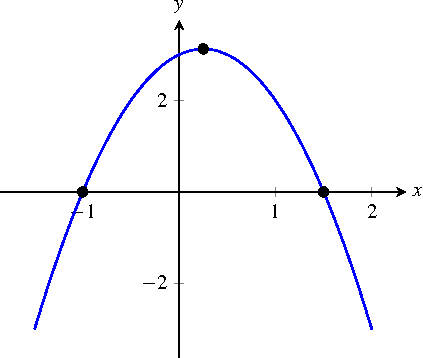
\includegraphics[scale=1]{image/07/aminus2-b1-c3.pdf}
\caption{%%
  Graph of the function $f(x) = -2x^2 + x + 3$.
}
\label{fig:aminus2_b1_c3}
\end{figure}
\end{solution}
}{}

\begin{exercise}
Sketch the graph of $f(x) = -x^2 + 1$.
\end{exercise}

\ifbool{showSolution}{
\begin{solution}
You have the values $a = -1$ and $c = 1$.  The value of $b$ is
$b = 0$ because $f(x) = -x^2 + 1 = -x^2 + 0x + 1$.  Again, you can use
three points to draw the graph of $f(x)$.  Those three points are: the
tip of the parabola and the two $x$-intercepts.

Use \Equation{eqn:parabola_tip_x_coordinate} to see that the tip point
occurs at the $x$-coordinate
\[
x
=
-\frac{0}{2(-1)}
=
0
\]
whose corresponding $y$-coordinate is
\[
y
=
f(0)
=
-0^2 + 1
=
1.
\]
Then the tip of the parabola occurs at the point $\tuple{0}{1}$.

Let's calculate the $x$-intercepts.  Use
\Equation{eqn:quadratic_formula} to obtain the $x$-intercept
%%
\begin{align*}
x
&=
\frac{
  -0 + \sqrt{0^2 - 4(-1)(1)}
}{
  2(-1)
} \\[4pt]
&=
\frac{
  \sqrt{4}
}{
  -2
} \\[4pt]
&=
-1.
\end{align*}
%%
The other $x$-intercept occurs at
%%
\begin{align*}
x
&=
\frac{
  -0 - \sqrt{0^2 - 4(-1)(1)}
}{
  2(-1)
} \\[4pt]
&=
\frac{
  -\sqrt{4}
}{
  -2
} \\[4pt]
&=
1.
\end{align*}
%%
Thus the $x$-intercepts are $\tuple{-1}{0}$ and $\tuple{1}{0}$.  Plot
the three points and connect the dots to obtain the graph in
\Figure{fig:aminus1_c1}.
\end{solution}

\begin{figure}[!htbp]
\centering
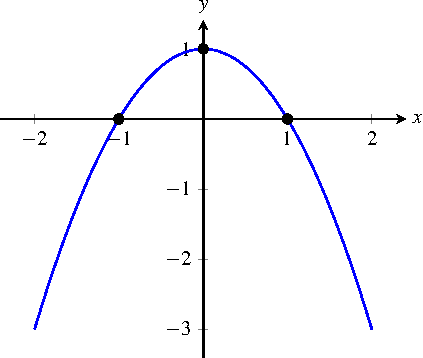
\includegraphics[scale=1]{image/07/aminus1-c1.pdf}
\caption{%%
  Graph of the function $f(x) = -x^2 + 1$ through three points.
}
\label{fig:aminus1_c1}
\end{figure}
}{}


%%%%%%%%%%%%%%%%%%%%%%%%%%%%%%%%%%%%%%%%%%%%%%%%%%%%%%%%%%%%%%%%%%%%%%%%%%%

\section{The discriminant}

You have seen in \Section{sec:quadratic_formula} how the quadratic
formula can help you to sketch the graph of a quadratic function.  The
general strategy was to determine the tip point of the parabola and
then use the quadratic formula to calculate two $x$-intercepts of the
function.  You plot the three points on one set of coordinate axes and
connect the dots to obtain a graph of the function.  But this strategy
does not always work.

To understand why the graph drawing strategy
from \Section{sec:quadratic_formula} can fail, let's consider the
example of the function $f(x) = x^2$.  According to the above
strategy, you first need to calculate the tip point.  This is easy
enough.  You have the values $a = 1$ and $b = c = 0$.  Just use
\Equation{eqn:parabola_tip_x_coordinate} to see that the
$x$-coordinate of the tip point is
%%
\begin{align*}
x
&=
-\frac{0}{2(1)} \\[4pt]
&=
0.
\end{align*}
%%
The corresponding $y$-coordinate is
%%
\begin{align*}
y
&=
f(0) \\[4pt]
&=
0^2 \\[4pt]
&=
0
\end{align*}
%%
and therefore the function $f(x) = x^2$ has its tip point at the
origin.  Now use the quadratic \Formula{eqn:quadratic_formula} to see
that the $x$-intercepts of $f(x)$ occur at the $x$-coordinate
%%
\begin{align*}
x
&=
\frac{
  -0 \pm \sqrt{0^2 - 4(1)(0)}
}{
  2(1)
} \\[4pt]
&=
\pm
\frac{
  \sqrt{0}
}{
  2
} \\[4pt]
&=
0
\end{align*}
%%
with the corresponding $y$-coordinate being $y = f(0) = 0$.  The
upshot is that the tip of $f(x)$ is also its $x$-intercept, i.e.~the
point $\tuple{0}{0}$.  The above strategy for graphing a quadratic
function results in only one point, not the three that you require.
In the case of the function $f(x) = x^2$, you should have used the
strategy from \Section{sec:general_form}.

\begin{exercise}
Consider the function $f(x) = x^2 + 2x + 1$.  Explain why the graph
drawing strategy from \Section{sec:quadratic_formula} cannot help you
with sketching the graph of $f(x)$.
\end{exercise}
%%
\ifbool{showSolution}{
\begin{solution}
First, let's calculate the tip point of the parabola.  From
\Equation{eqn:parabola_tip_x_coordinate}, the $x$-coordinate of the
tip point is
%%
\begin{align*}
x
&=
-\frac{2}{2(1)} \\[4pt]
&=
-1.
\end{align*}
%%
The corresponding $y$-coordinate is $y = f(-1) = 0$.  The tip of the
parabola is located at the point $\tuple{-1}{0}$.

Next, you use the quadratic \Formula{thm:quadratic_formula} to
determine the $x$-intercepts of $f(x)$.  The $x$-coordinates of the
$x$-intercept are
%%
\begin{align*}
x
&=
\frac{
  -2 \pm \sqrt{2^2 - 4(1)(1)}
}{
  2(1)
} \\[4pt]
&=
\frac{
  -2 \pm \sqrt{4 - 4}
}{
  2
} \\[4pt]
&=
\frac{-2}{2} \\[4pt]
&=
-1.
\end{align*}
%%
The corresponding $y$-coordinate is $y = f(-1) = 0$.  In other words,
the function $f(x)$ has its $x$-intercepts at the point
$\tuple{-1}{0}$, which is also the tip point of the parabola.  In the
case of $f(x)$, the graph sketching strategy
from \Section{sec:quadratic_formula} results in only one point, not
the three that you need to draw the graph.
\end{solution}
}{}

Is there a way to determine when to use the strategies
from \Sections{sec:general_form}{sec:quadratic_formula} for graphing a
quadratic function?  The answer is yes, but you need to understand a
number called the \emph{discriminant} of a quadratic function.

\begin{definition}
\label{def:discriminant}
\textbf{Discriminant.}
Let $\triple{a}{b}{c} \in \RR$ such that $a \neq 0$ and consider the
quadratic function $f(x) = ax^2 + bx + c$.  If the roots of $f(x)$ are
\[
x
=
\frac{
  -b \pm \sqrt{b^2 - 4ac}
}{
  2a
}
\]
then the number $\Delta = b^2 - 4ac$ is called the \emph{discriminant}
of $f(x)$.
\end{definition}

Like any real number, the discriminant can take on one of three types
of values.  The discriminant can be either negative, zero, or
positive.  Depending on the value of the discriminant, a quadratic
function will have either zero, one, or two $x$-intercepts.  Let's
consider each of the three cases separately.  Suppose $f(x)$ is a
quadratic function whose discriminant is $\Delta$.

\begin{packedenumeral}
\item If $\Delta < 0$, then $f(x)$ does not intersect the $x$-axis.
  The graph of $f(x)$ lies wholly above or below the $x$-axis.  See
  \Figure{fig:negative_discriminant}.

\item If $\Delta = 0$, then $f(x)$ intersects the $x$-axis once.  The
  point of intersection is also the tip point of the quadratic
  function.  This case is illustrated in
  \Figure{fig:zero_discriminant}.

\item If $\Delta > 0$, then $f(x)$ has two different $x$-intercepts.
  See \Figure{fig:positive_discriminant}.
\end{packedenumeral}

\begin{figure}[!htbp]
\centering
\subfigure[]{
  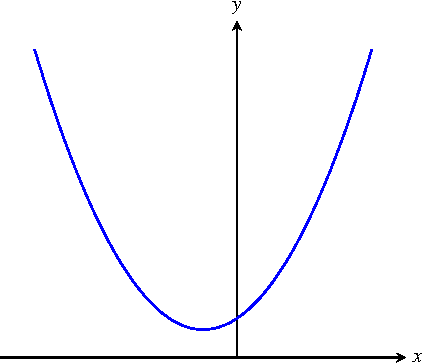
\includegraphics[scale=0.85]{image/07/a2-b1-c1.pdf}
}
%%
\quad
%%
\subfigure[]{
  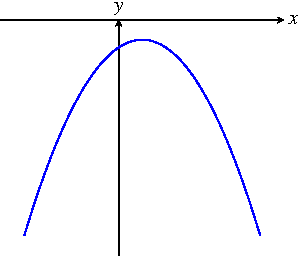
\includegraphics[scale=0.93]{image/07/aminus2-b1-cminus2.pdf}
}
\caption{%%
  When the discriminant is negative, the graph of a quadratic function
  does not intersect the $x$-axis.
}
\label{fig:negative_discriminant}
\end{figure}

\begin{figure}[!htbp]
\centering
\subfigure[]{
  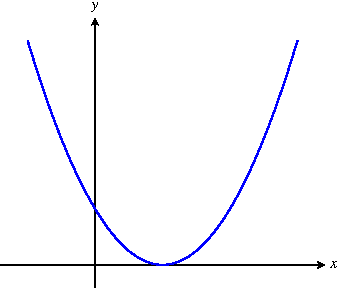
\includegraphics[scale=1]{image/07/a1-bminus2-c1.pdf}
}
%%
\qquad
%%
\subfigure[]{
  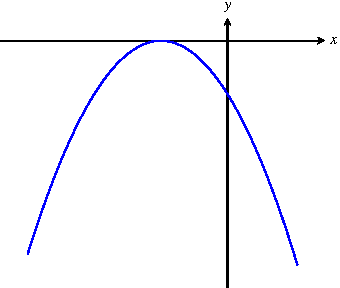
\includegraphics[scale=1]{image/07/aminus9quarter-bminus3-cminus1.pdf}
}
\caption{%%
  When the discriminant is zero, the graph of a quadratic function
  intersects the $x$-axis at exactly one point.
}
\label{fig:zero_discriminant}
\end{figure}

\begin{figure}[!htbp]
\centering
\subfigure[]{
  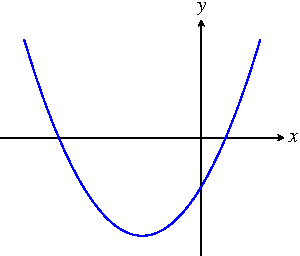
\includegraphics[scale=1]{image/07/a1-b2-cminus1.pdf}
}
%%
\qquad
%%
\subfigure[]{
  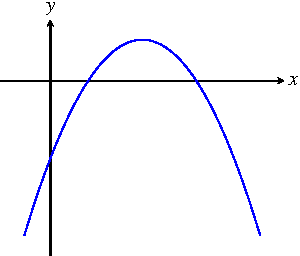
\includegraphics[scale=1]{image/07/aminus1-b3half-cminus2.pdf}
}
\caption{%%
  When the discriminant is positive, the graph of a quadratic function
  intersects the $x$-axis at two different points.
}
\label{fig:positive_discriminant}
\end{figure}

What all this means is that if the discriminant of a quadratic
function $f(x)$ is either negative or zero, then you should use the
strategy from \Section{sec:general_form} to sketch the graph of
$f(x)$.  If the discriminant of $f(x)$ is positive, then the strategy
from \Section{sec:quadratic_formula} can be used to draw the graph of
$f(x)$.  Or you could forget about \Section{sec:quadratic_formula}
entirely and use the technique from \Section{sec:general_form} because
the graph drawing strategy from that section will always work for any
quadratic function.  So why would you bother to learn about the
discriminant?

An answer can be found in
\Problems{prob:zero_discriminant}{prob:positive_discriminant} and can
be summarised as follows.  The discriminant of a quadratic function
$f(x)$ tells you how many roots $f(x)$ has.  You do not need to use
the quadratic \Formula{eqn:quadratic_formula} to know that $f(x)$ has
either a unique root or two different roots or that the graph of
$f(x)$ does not intersect the $x$-axis.  All you need to do is
calculate the discriminant of $f(x)$, which is much simpler to do than
calculating the actual roots of $f(x)$.

\begin{example}
Explain why the quadratic function $f(x) = 2x^2 + x + 1$ does not
intersect the $x$-axis.
\end{example}

\begin{solution}
The discriminant of $f(x)$ is
$\Delta = 1^2 - 4(2)(1) = 1 - 8 = -7$.  Since $\Delta$ is negative,
the graph of $f(x)$ does not intersect the $x$-axis.
\end{solution}

\begin{exercise}
How many unique roots does the function $f(x) = x^2 - 2x + 1$ have?
\end{exercise}
%%
\ifbool{showSolution}{
\begin{solution}
The discriminant of $f(x)$ is
$\Delta = (-2)^2 - 4(1)(1) = 4 - 4 = 0$.  Therefore $f(x)$ has a
unique root.
\end{solution}
}{}

\begin{exercise}
Explain why $f(x) = -x^2 - \frac{7}{2}x - 2$ has two different roots.
\end{exercise}
%%
\ifbool{showSolution}{
\begin{solution}
The discriminant of $f(x)$ is
$\Delta
=
\parenthesis*{-\frac{7}{2}}^2 - 4(-1)(-2)
=
\frac{49}{4} - 8$,
which is a positive number because $\Delta = 17/4$.  Therefore $f(x)$
has two different roots.
\end{solution}
}{}


%%%%%%%%%%%%%%%%%%%%%%%%%%%%%%%%%%%%%%%%%%%%%%%%%%%%%%%%%%%%%%%%%%%%%%%%%%%

\section{Applications}

This section will show you how the quadratic function can be used in a
variety of situations.  The section consists of mostly worked examples
and exercises.

\begin{example}
\label{ex:fence_a_rectangular_region}
You want to put a fence around a rectangular region that has an area
of $7$ metres squared.  You want the length of the rectangular region
to be two metres longer than the width.  Calculate the width of the
region.
\end{example}

\begin{solution}
Whenever possible, you should first draw a picture to help you solve a
problem.  In this example, the rectangular region and its dimensions
can be illustrated as shown in
\Figure{fig:rectangular_region_7_metres_squared}.  Since the width of
the region is $w$ metres and its length is $w + 2$ metres, the area of
the region is $(w + 2)w$ metres squared.  However, you also know that
the region has an area of $7$~metres squared, which can be used to
give you the equation
%%
\begin{equation}
\label{eqn:rectangular_region_equation}
(w + 2)w
=
7.
\end{equation}

\begin{figure}[!htbp]
\centering
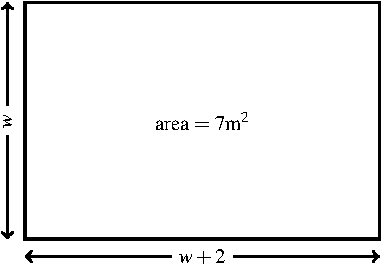
\includegraphics[scale=1]{image/07/rectangular-fence.pdf}
\caption{%%
  A rectangular region whose area is $7$ metres squared.  The width of
  the region is denoted $w$.
}
\label{fig:rectangular_region_7_metres_squared}
\end{figure}

Let's determine all values of $w$ that satisfy
\Equation{eqn:rectangular_region_equation}.  Expand the left-hand side
of \Equation{eqn:rectangular_region_equation} to get $w^2 + 2w = 7$.
Upon moving everything to the left-hand side, you end up with the
quadratic equation
%%
\begin{equation}
\label{eqn:rectangular_region_quadratic}
w^2 + 2w - 7
=
0.
\end{equation}
%%
Writing the left-hand side as $f(w) = w^2 + 2w - 7$,
\Equation{eqn:rectangular_region_quadratic} can also be written as
$f(w) = 0$.  This means that you want to determine all roots of
$f(w)$.  Before calculating the roots of $f(w)$, you investigate
whether $f(w)$ has a unique root, two different roots, or the graph of
$f(w)$ does not intersect the horizontal axis.  This is a job for the
discriminant.  The discriminant of $f(w)$ is $\Delta = 32$.  This is a
positive number so there exists at least one real value of $w$ that
solves \Equation{eqn:rectangular_region_equation}.  Using the
quadratic formula, the roots of $f(w)$ can be written as
$w = -1 \pm 2\sqrt{2}$.  One root of $f(w)$ is given by
\[
w_1
=
2\sqrt{2} - 1
\]
which is positive.  The other root is given by
\[
w_2
=
-2\sqrt{2} - 1
\]
which is negative.  You reject the number $w_2$ because the width of
the rectangular region cannot be a negative number.  To confirm your
decision to reject the root $w_2$, you sketch the graph of $f(w)$ as
shown in \Figure{fig:rectangular_region_quadratic_roots} and note that
$w_2$ is located on the negative half of the $w$-axis, i.e.~the
horizontal axis.  You conclude that the width of the rectangular
region is approximately $2\sqrt{2} - 1 \approx 1.8284$ metres long,
rounded to four decimal places.
\end{solution}

\begin{figure}[!htbp]
\centering
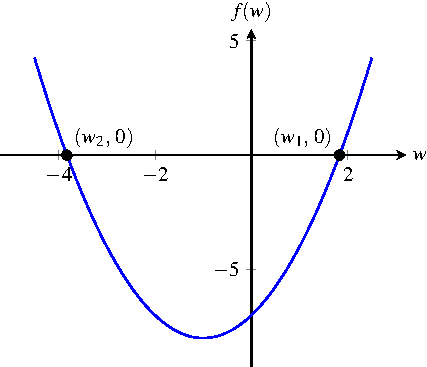
\includegraphics[scale=1]{image/07/a1-b2-cminus7.pdf}
\caption{%%
  Graph of the function $f(w) = w^2 + 2w - 7$.  The two dots indicate
  the two different roots of $f(w)$.
}
\label{fig:rectangular_region_quadratic_roots}
\end{figure}

\begin{exercise}
\label{ex:rectangular_region_discriminant}
In the solution of \Example{ex:fence_a_rectangular_region}, verify
that the discriminant is $\Delta = 32$.
\end{exercise}
%%
\ifbool{showSolution}{
\begin{solution}
In the equation $f(w) = w^2 + 2w - 7$, you have the values $a = 1$,
$b = 2$, and $c = -7$.  Use \Definition{def:discriminant} to see that
the discriminant of $f(w)$ is
%%
\begin{align*}
\Delta
&=
2^2 - 4(1)(-7) \\[4pt]
&=
4 + 28 \\[4pt]
&=
32
\end{align*}
%%
as required.
\end{solution}
}{}

\begin{exercise}
In the solution of \Example{ex:fence_a_rectangular_region}, verify
that the roots of $f(w)$ can be written as $w = -1 \pm 2\sqrt{2}$.
\end{exercise}
%%
\ifbool{showSolution}{
\begin{solution}
You have the equation $f(w) = w^2 + 2w - 7$, whose roots can be
calculated by using the quadratic formula.  The discriminant of $f(w)$
is known to be $\Delta = 32$, as verified in
\Exercise{ex:rectangular_region_discriminant}, so the roots are
%%
\begin{align*}
w
&=
\frac{
  -2 \pm \sqrt{\Delta}
}{
  2(1)
} \\[4pt]
&=
\frac{
  -2 \pm \sqrt{2 \times 4^2}
}{
  2
} \\[4pt]
&=
\frac{
  -2 \pm 4\sqrt{2}
}{
  2
} \\[4pt]
&=
\frac{
  2(-1 \pm 2\sqrt{2})
}{
  2
} \\[4pt]
&=
-1 \pm 2\sqrt{2}
\end{align*}
%%
as required.
\end{solution}
}{}

\begin{example}
\label{ex:running_ants}
Two ants are next to each other.  Ant $A$ runs eastward at a rate of
two centimetres per second.  After one second since ant $A$ started
running, ant $B$ runs northward also at the same rate.  How long since
ant $A$ started running does it take for both ants to be five
centimetres apart?
\end{example}

\begin{solution}
As in \Example{ex:fence_a_rectangular_region}, you should first try to
draw a picture that can help you in solving the problem.  Denote by
$t$ the time in seconds and use $t$ to represent the amount of time
that ant $A$ runs.  Since ant $A$ runs in the eastern direction at two
centimetres per second, after $t$ seconds the ant would have covered a
horizontal distance of $2t$ centimetres.  When ant $A$ starts running,
ant $B$ is still at the starting position and must wait one second
before it starts to run in the northern direction.  The amount of time
that ant $B$ runs is one second less than the amount of time that ant
$A$ runs.  In other words, the duration of time that ant $B$ runs can
be written as $t - 1$ seconds, after which the ant would have
travelled a vertical distance of $2(t - 1)$ centimetres.  The
situation is illustrated in \Figure{fig:running_ants_triangle}.

\begin{figure}[!htbp]
\centering
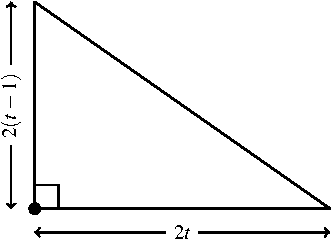
\includegraphics[scale=1]{image/07/running-ants.pdf}
\caption{%%
  A right-angled triangle that represents the directions in which two
  ants run.  The dot indicates the starting position of the ants.  The
  variable $t$ denotes time in seconds.  After $t$ seconds, the
  distance between the ants is represented by the length of the
  hypotenuse.
}
\label{fig:running_ants_triangle}
\end{figure}

Let's now formulate the problem as an equation.  The horizontal and
vertical distances travelled by both ants can be represented as the
base and height, respectively, of the right-angled triangle in
\Figure{fig:running_ants_triangle}.  After $t$ seconds have passed,
the distance between the ants is represented by the length of the
hypotenuse of the triangle.  Using Pythagoras' theorem, the problem
can be formulated as the quadratic equation
%%
\begin{equation}
\label{eqn:running_ants_quadratic_equation}
8t^2 - 8t + 4
=
25.
\end{equation}

The problem now is to determine all values of $t$ that satisfy
\Equation{eqn:running_ants_quadratic_equation}.  Note that the
equation can also be written as
\[
8t^2 - 8t - 21
=
0.
\]
Writing $f(t) = 8t^2 - 8t - 21$,
\Equation{eqn:running_ants_quadratic_equation} is equivalent to the
equation $f(t) = 0$, hence the values of $t$ that satisfy
\Equation{eqn:running_ants_quadratic_equation} are the same as the
roots of $f(t)$.  The quadratic formula shows that the roots of $f(t)$
are
%%
\begin{equation}
\label{eqn:running_ants_roots}
t_1
=
\frac{1}{2}
+
\frac{\sqrt{46}}{4}
%%
\qquad
\text{and}
\qquad
%%
t_2
=
\frac{1}{2}
-
\frac{\sqrt{46}}{4}.
\end{equation}
%%
You reject the root $t_2$ because it is negative.  A negative value of
time does not make sense in the context of the problem.  Therefore the
ants would be five centimetres apart after approximately
$\frac{1}{2}
+
\frac{\sqrt{46}}{4}
\approx
2.1956$
seconds~(rounded to four decimal places) since ant $A$ started running.
\end{solution}

\begin{exercise}
Explain why \Example{ex:running_ants} can be represented as
\Equation{eqn:running_ants_quadratic_equation}.
\end{exercise}
%%
\ifbool{showSolution}{
\begin{solution}
From \Figure{fig:running_ants_triangle} you know that after $t$
seconds, ant $A$ would have travelled $2t$ centimetres and ant $B$
would have travelled $2(t - 1)$ centimetres.  These numbers are the
base and height, respectively, of a right-angled triangle.  After $t$
seconds, the distance between the ants is represented by the  length
of the hypotenuse in \Figure{fig:running_ants_triangle}.  You want to
know when the ants are $5$ centimetres apart, so the hypotenuse is $5$
centimetres.  By Pythagoras' theorem, the three sides of the
right-angled triangle are related by the equation
\[
(2t)^2 + \bigparen{2 (t - 1)}^2
=
5^2.
\]
Upon expanding the parentheses, the equation can be written as
\[
4t^2 + (2t - 2)^2
=
25.
\]
Expand the remaining pair of parentheses to get
\[
4t^2 + 4t^2 - 8t + 4
=
25.
\]
After collecting like terms, you end up with
\Equation{eqn:running_ants_quadratic_equation}.
\end{solution}
}{}

\begin{exercise}
In the solution to \Example{ex:running_ants}, verify that the roots of
$f(t)$ are those given by~\eqref{eqn:running_ants_roots}.
\end{exercise}
%%
\ifbool{showSolution}{
\begin{solution}
You have the quadratic function $f(t) = 8t^2 - 8t - 21$.  Using the
quadratic formula, the roots of $f(t)$ are
%%
\begin{align*}
t
&=
\frac{
  -(-8) \pm \sqrt{(-8)^2 - 4(8)(-21)}
}{
  2(8)
} \\[4pt]
&=
\frac{
  8 \pm \sqrt{736}
}{
  16
} \\[4pt]
&=
\frac{
  8 \pm \sqrt{4^2 \times 2 \times 23}
}{
  16
} \\[4pt]
&=
\frac{
  8 \pm 4\sqrt{46}
}{
  16
} \\[4pt]
&=
\frac{
  4 \parenthesis*{2 \pm \sqrt{46}}
}{
  4^2
} \\[4pt]
&=
\frac{
  2 \pm \sqrt{46}
}{
  4
} \\[4pt]
&=
\frac{1}{2}
\pm
\frac{\sqrt{46}}{4}
\end{align*}
%%
which are the same as those given by~\eqref{eqn:running_ants_roots}.
\end{solution}
}{}


%%%%%%%%%%%%%%%%%%%%%%%%%%%%%%%%%%%%%%%%%%%%%%%%%%%%%%%%%%%%%%%%%%%%%%%%%%%

\subsection*{Free fall}

You throw a ball straight up into the air.  The ball travels upward
for some time, reaches a maximum height, and then falls to the
ground.  Other than throwing the ball upward, you do not interfere
with the movement of the ball, but allow the forces of gravity and air
drag~(air resistance) to act on the ball.  In many cases, the force of
air drag can be ignored.  For now you only need to take into account
the force of gravity.  When the ball is allowed to move upward and
downward freely as described above, the motion of the ball is an
example of \emph{free fall}.

The position of the ball changes with time.  But precisely in what
way?  To analyse the position of the ball, let's make various
assumptions.  Denote by $t$ the time in seconds and let $f(t)$ be the
height in metres of the ball.  The \emph{initial height} of the ball
is the ball's height above ground level before the ball moves upward.
When you hold the ball in your hand just before you throw it upward,
the initial height of the ball is the distance~(in metres) from your
hand to the ground.  If the ball is on the ground before it moves
upward, its initial height is zero metres.  Let $h$ be the initial
height of the ball.  The \emph{initial velocity} of the ball is the
speed in metres per second with which the ball is thrown upward.
Denote the initial velocity of the ball by $v$.  The force of gravity
acts on the ball in a downward manner.  This is because gravity tends
to pull an object downward towards the centre of the Earth.  The force
of gravity is usually written as $g$ and its value is the constant of
$9.8$ metres per second squared.  To analyse the position of the ball,
you must take into account the initial height of the ball, the upward
distance it travels as time passes, and the downward force of gravity.
The position of the ball above ground level can be approximated by the
quadratic function
%%
\begin{equation}
\label{eqn:position_of_object_under_free_fall}
f(t)
=
-\frac{1}{2} gt^2 + vt + h.
\end{equation}

\begin{example}
\label{ex:spring_ball}
A spring is located at ground level and can shoot a ball upward at an
initial velocity of $10$ metres per second.
%%
\begin{packedenum}
\item\label{ex:spring_ball_graph}
  Write down a function for the position of the ball and graph the
  function.

\item\label{ex:spring_ball_time_to_maximum_height}
  Determine the amount of time~(in seconds) required for the ball to
  reach maximum height.  Calculate the maximum height~(in metres) that
  the ball reaches.

\item\label{ex:spring_ball_time_hit_ground}
  When will the ball reach the ground?
\end{packedenum}
\end{example}

\begin{solution}
\solutionpart{ex:spring_ball_graph}
You know that the force of gravity is $g = 9.8$ metres per second
squared.  The initial velocity is $v = 10$ metres per second.  Since
the spring is located at ground level, let's assume that the initial
height of the ball is $h = 0$ metres.  Substitute these values into
\Equation{eqn:position_of_object_under_free_fall} and simplify the
result to get $f(t) = -\frac{49}{10}t^2 + 10t$, whose graph is shown
in \Figure{fig:spring_ball_graph}.  This is a rough sketch that
illustrates three points on which you should concentrate.  First is
the point at the origin $\tuple{0}{0}$ that tells you the initial
height of the ball at time $t = 0$ before the ball is shot upward.
Next is the tip point, which in this example is the highest point
$\tuple{a}{f(a)}$ of the graph of $f(t)$.  The tip point
$\tuple{a}{f(a)}$ tells you that the ball reaches its maximum height
of $f(a)$ metres above the ground at time $t = a$ seconds after being
shot upward by the spring.  The third point $\tuple{b}{0}$ tells you
approximately how long the ball is in the air before it lands on the
ground.  You do not yet know the values of $a$ and $b$.  This is just
a rough sketch to help you understand the example.

\begin{figure}[!htbp]
\centering
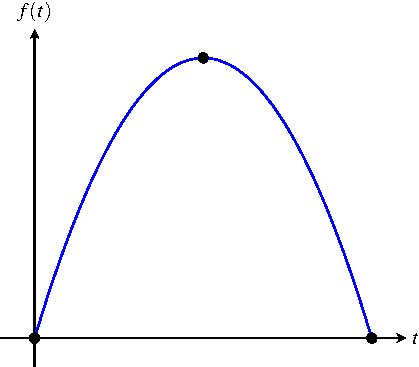
\includegraphics[scale=1]{image/07/spring-ball.pdf}
\caption{%%
  The height of a ball as a function of time.  Here, time $t$ is
  measured in seconds and the height $f(t)$ of the ball is measured in
  metres above the ground.
}
\label{fig:spring_ball_graph}
\end{figure}

\solutionpart{ex:spring_ball_time_to_maximum_height}
From \Formula{eqn:parabola_tip_x_coordinate} you know that the tip
point~(i.e. highest point) of the graph of $f(t)$ occurs at
$t = 50/49$.  This means that the ball reaches its maximum height
above the ground at approximately $t = 50/49 \approx 1.0204$
seconds~(rounded to four decimal places) after being shot up by the
spring.  The maximum height that the ball reaches is
$f(50 / 49) = 250 / 49$, which is approximately $5.1020$ metres above
the ground, rounded to four decimal places.

\solutionpart{ex:spring_ball_time_hit_ground}
You can use the quadratic formula to calculate the time at which the
ball hits the ground.  However, the following is a simple method that
does not use the quadratic formula.  Note that the function $f(t)$ can
be factorised as
%%
\begin{align*}
f(t)
&=
-\frac{49}{10} t^2 + 10t \\[4pt]
&=
\parenthesis*{-\frac{49}{10} t + 10} t \\[4pt]
&=
\parenthesis*{10 - \frac{49}{10} t} t.
\end{align*}
%%
Since the roots of $f(t)$ are those values of $t$ such that the
equation $f(t) = 0$ is true, this is the same as determining the
values of $t$ such that the following equation is true:
%%
\begin{equation}
\label{eqn:spring_ball_equation_factored}
\parenthesis*{10 - \frac{49}{10} t} t
=
0.
\end{equation}
%%
Equation~\eqref{eqn:spring_ball_equation_factored} is true when
$t = 0$.  However, the point $\tuple{0}{0}$ is the starting position
of the ball when it is initially on the ground.  So you can ignore the
root $t = 0$ of $f(t)$.  If the factor $10 - \frac{49}{10} t = 0$,
then \Equation{eqn:spring_ball_equation_factored} will also be true.
You must solve the equation $10 - \frac{49}{10} t = 0$ for $t$.  Doing
so gives you the root $t = 100 / 49$.  Therefore the ball will reach
the ground at approximately $t = 100 / 49 \approx 2.0408$ seconds
after being shot up by the spring.
\end{solution}

\begin{exercise}
In the solution of \Subexample{ex:spring_ball}{ex:spring_ball_graph},
verify that the height~(above the ground) of the ball can be written
as $f(t) = -\frac{49}{10} t^2 + 10t$.
\end{exercise}
%%
\ifbool{showSolution}{
\begin{solution}
You have the values $g = 9.8 = 49/5$, $v = 10$, and $h = 0$.
Substitute these values into
\Equation{eqn:position_of_object_under_free_fall} to obtain
%%
\begin{align*}
f(t)
&=
-\frac{49}{5} \times \frac{1}{2} t^2 + 10t + 0 \\[4pt]
&=
-\frac{49}{10} t^2 + 10t
\end{align*}
%%
as required.
\end{solution}
}{}


%%%%%%%%%%%%%%%%%%%%%%%%%%%%%%%%%%%%%%%%%%%%%%%%%%%%%%%%%%%%%%%%%%%%%%%%%%%

\section*{Problem}

\begin{problem}
\item\label{prob:zero_discriminant}
  Let $f(x)$ be a quadratic function whose discriminant is zero.
  %%
  \begin{packedenum}
  \item\label{subprob:zero_discriminant_unique_root}
    Prove that $f(x)$ has a unique root.

  \item\label{subprob:zero_discriminant_root_is_tip_point}
    Prove that the root of $f(x)$ is also the tip point of the
    parabola.
  \end{packedenum}
\ifbool{showSolution}{
\begin{solution}
\solutionpart{subprob:zero_discriminant_unique_root}
Suppose the quadratic function $f(x)$ can be written as
$f(x) = ax^2 + bx + c$, where $\triple{a}{b}{c} \in \RR$ such that
$a \neq 0$.  You need to show that there is only one value of $x$ such
that $f(x) = 0$.  By \Theorem{thm:quadratic_formula} the roots of
$f(x)$ are
\[
x
=
\frac{
  -b \pm \sqrt{b^2 - 4ac}
}{
  2a
}
\]
where the number $\Delta = b^2 - 4ac$ is the discriminant of $f(x)$.
Since the discriminant is $\Delta = 0$, then the roots of $f(x)$ can
be written as
%%
\begin{align*}
x
&=
\frac{
  -b \pm \sqrt{0}
}{
  2a
} \\[4pt]
&=
\frac{-b \pm 0}{2a} \\[4pt]
&=
-\frac{b}{2a}
\end{align*}
%%
which is one number.  Therefore $f(x)$ has a unique root.

\solutionpart{subprob:zero_discriminant_root_is_tip_point}
From \Equation{eqn:parabola_tip_x_coordinate}, the tip of the parabola
occurs at the $x$-coordinate $x = -b/2a$, which
from \Part{subprob:zero_discriminant_unique_root} is also the unique
root of $f(x)$.
\end{solution}
}{}

\item\label{prob:positive_discriminant}
  If $f(x)$ is a quadratic function with positive discriminant, prove
  that $f(x)$ has two different roots.
\ifbool{showSolution}{
\begin{solution}
Suppose that the quadratic function $f(x)$ can be written as
$f(x) = ax^2 + bx + c$, where $\triple{a}{b}{c}$ are real numbers such
that $a \neq 0$.  Use \Theorem{thm:quadratic_formula} to write the
roots of $f(x)$ as
\[
x
=
\frac{
  -b \pm \sqrt{b^2 - 4ac}
}{
  2a
}.
\]
As the discriminant is assumed to be positive, the number
$\Delta = b^2 - 4ac$ is positive and so the square root
$\sqrt{\Delta}$ is also positive.  Thus the roots of $f(x)$ can be
written as
\[
x
=
\frac{-b + \sqrt{\Delta}}{2a}
%%
\qquad
\text{and}
\qquad
%%
x
=
\frac{-b - \sqrt{\Delta}}{2a}
\]
which are two different numbers because $\sqrt{\Delta} > 0$.
\end{solution}
}{}

\item If $a$ is any real number, its square root can be written as
  $\sqrt{a} = a^{1/2}$.  Explain what is wrong with the following
  expression:
  %%
  \begin{align*}
  1
  &=
  \sqrt{1} \\[4pt]
  &=
  \sqrt{(-1)^2} \\[4pt]
  &=
  \bigparen{(-1)^2}^{1/2} \\[4pt]
  &=
  (-1)^{2/2} \\[4pt]
  &=
  (-1)^1 \\[4pt]
  &=
  -1.
  \end{align*}
\ifbool{showSolution}{
\begin{solution}
The number $\sqrt{(-1)^2}$ is the distance between the points
$\tuple{0}{0}$ and $\tuple{-1}{0}$.  This is because you have
%%
\begin{align*}
\sqrt{
  (0 - 0)^2 + (-1 - 0)^2
}
&=
\sqrt{0^2 + (-1)^2} \\[4pt]
&=
\sqrt{(-1)^2}.
\end{align*}
%%
As the distance cannot be negative, you must first simplify the
expression $(-1)^2$ before you take its square root.
\end{solution}
}{}
\end{problem}

\end{document}
